\section{Introducción}
\label{IntroduccionConcurrencia}

``La idea de programación concurrente siempre estuvo asociada al mundo de los
\textit{Sistemas Operativos}. No en vano, los primeros programas concurrentes
fueron los propios Sistemas Operativos de multiprogramación en los que un solo
procesador debía repartir su tiempo entre muchos usuarios.''\cite{PalmaConcurrente}

En las últimas dos décadas, la programación concurrente ganó gran interés y
actualmente está presente en la mayoría de las aplicaciones.
Esto se debe principalmente a algunos grandes hitos en la programación:
\begin{itemize}
	\item La aparición del concepto de \textit{hilo} o \textit{thread}. Permiten la
	ejecución de programas de manera más rápida y eficiente que los programas
	basados en procesos.
	\item La aparición de lenguajes de alto nivel con soporte nativo para
	programación de hilos y de procesos.
	\item La aparición de internet, entorno donde la concurrencia se hace necesaria
	en todo aspecto.
	\item El desarrollo y gran avance de hardware capaz de ejecutar múltiples hilos
	y procesos de forma paralela. Esto permite aprovechar las ventajas de
	performance de la concurrencia. Las principales arquitecturas capaces de
	explotar el paralelismo a nivel de hilo y/o de proceso son
	\begin{itemize}
	    \item Procesadores Multi-Core
	    \item Procesadores Many-Core
	    \item Procesadores con soporte Multi-Thread
    \end{itemize}
\end{itemize}

\section{Programación Concurrente}
\label{ProgramacionConcurrente}

La \textit{programación concurrente} es la disciplina que se encarga del estudio
de las notaciones que permiten especificar la ejecución concurrente de las
acciones de un programa, así como resolver los problemas inherentes a la
ejecución concurrente (ver \ref{ProblemasConcurrencia}). Es de interés
formalizar el concepto de ejecución concurrente y de ejecución paralela a fin
de poder diferenciarlos:

\begin{itemize}
	\stepcounter{definitionsCounter}
	\item [\underline{Definición \thedefinitionsCounter :} ] Dos procesos
	o hilos son \textit{concurrentes} si la primera instrucción de uno de ellos se
	ejecuta después de la primera del otro y antes de la última.
	\stepcounter{definitionsCounter}
	\item [\underline{Definición \thedefinitionsCounter :} ] Dos procesos o hilos
	se están ejecutando de manera \textit{paralela} si son concurrentes y la
	ejecución de ambos se da al mismo tiempo.
\end{itemize}

Para que dos procesos sean concurrentes no es necesario que se ejecuten al mismo
tiempo, es suficiente que exista un intercalado entre la ejecución de sus
instrucciones. En este proyecto integrador, es de interés fundamentalmente la
ejecución concurrente.

Anteriormente en esta sección se mencionó que existen problemas aparejados a la
programación de sistemas concurrentes. Sabiendo esto resulta necesario conocer
las ventajas de la programación concurrente, que justifiquen su uso por encima de
las dificultades que genera.

\subsection{Ventajas de la Programación Concurrente}

Los beneficios de programar de manera concurrente pueden englobarse en tres
categorías:

\begin{itemize}
	\item \underline{Incremento en la velocidad de ejecución:} Cuando se ejecuta un
	programa concurrente en un entorno multiprocesador, los distintos procesos que
	lo forman pueden ejecutarse de manera paralela, con lo que el tiempo total de
	ejecución se reduce. Esto es especialmente ventajoso en programas de cálculo
	numérico.
	\item \underline{Solución de problemas inherentemente concurrentes:} Existen
	problemas cuya naturaleza es concurrente, por lo que un modelo de programación
	de este tipo se adapta más naturalmente a la resolución de estos problemas.
	\item \underline{Mejor aprovechamiento del tiempo de CPU:} Un sistema operativo
	con un ambiente de multiprogramación que permita la concurrencia es capaz de
	desalojar a un proceso que está esperando por un evento y no está haciendo uso
	del procesamiento de la CPU para brindarle este tiempo a otro proceso que lo
	requiera.
\end{itemize}

\subsection{Problemas y Propiedades de la Concurrencia}
\label{ProblemasConcurrencia}

Como se introdujo en la sección \ref{ProgramacionConcurrente}, existen
problemas que aparecen al programar de manera concurrente. Esto lleva a que los
programas concurrentes deban satisfacer una serie de propiedades (además de su
especificación técnica del dominio del problema) para funcionar correctamente.

Estas propiedades se dividen en dos grupos:

\subsubsection*{Propiedades de Seguridad}
Las propiedades de seguridad aseguran que ``nada malo'' va a pasar en la
ejecución del programa \cite{PalmaConcurrente}.
Estas son:

\begin{itemize}
    \item \underline{Exclusión Mutua:} Existen recursos que no pueden ser
    accedidos concurrentemente para evitar problemas de coherencia. Por esto se
    debe garantizar que a lo sumo un proceso está accediendo a un recurso de este
    tipo en un instante dado.
    \item \underline{Condición de Sincronización:} Se pueden dar situaciones
    donde un proceso debe esperar la ocurrencia de un evento para poder
    continuar su flujo. Ante estos casos se debe garantizar que el proceso
    espere por dicha ocurrencia, de otro modo el resultado puede ser indefinido
    o inesperado.
    \item \underline{Interbloqueo \textit{(Deadlock)}:} Sucede cuando dos o más
    procesos están esperando a que suceda un evento que nunca ocurrirá para continuar sus
    flujos de ejecución. El evento no ocurre porque las condiciones para que
    suceda están bloqueadas por los propios procesos.\\
    Para que el interbloqueo suceda efectivamente se tienen que cumplir las
    siguientes condiciones:
    \begin{itemize} 
        \item Exclusión Mutua: si no se exige exlusión mutua, no puede haber
        interdependencia entre los procesos.
        \item Retención y Espera: cada proceso debe retener un recurso y esperar
        a que se libere otro.
        \item No Apropiación: no se puede forzar a un proceso a que desaloje un
        recurso
        \item Circulo Vicioso de Espera: Se forma una cadena cerrada de
        procesos, donde cada uno retiene al menos un recurso que necesita el
        próximo proceso de la cadena.
    \end{itemize}
    Las tres primeras condiciones son necesarias pero no suficientes para que
    efectivamente ocurra el interbloqueo. La cuarta condición nace como
    consecuencia de las tres primeras, siempre que se produzca una secuencia de
    eventos que desemboque en un círculo de espera irresoluble.
    \cite{SistOpStallings}
\end{itemize}

\subsubsection*{Propiedades de Vivacidad}

Si se aseguran las propiedades de vivacidad, ``algo bueno'' pasará evantualmente
en la ejecución del programa.

\begin{itemize}
    \item \underline{Interbloqueo Activo \textit{(Livelock)}:} Se produce un
    interbloqueo activo cuando un sistema ejecuta una serie de instrucciones sin hacer ningún
    progreso. Esto se da cuando $N$ procesos necesitan $N$ recursos y se los
    intercambian sin obtener nunca el conjunto completo.
    \item \underline{Inanición \textit{(Starvation)}:} Se da cuando al menos una
    parte del sistema nunca recibe los recursos necesarios para continuar, o demora demasiado
    tiempo en recibirlos. No es necesario que todo el sistema se bloquee para
    estar en una situación de inanición.
\end{itemize}

\section{Mecanismos de Sincronización}

A fin de garantizar el cumplimiento de las propiedades introducidas en la
sección \ref{ProblemasConcurrencia}, es necesario sincronizar la ejecución de
los hilos/procesos. De lo contrario, se puede caer en problemas de coherencia y
consistencia de datos, o corrupción de los sistemas.

\subsection{Cooperación vs Competencia}

La sincronización de procesos se puede implementar basada en dos principios:
\begin{itemize}
    \item \underline{Cooperación:} Los procesos se comunican entre ellos para
    cooperar en la compartición de recursos. A su vez, existen dos tipos de
    cooperación:
    \begin{itemize}
        \item \underline{Cooperación por Compartición:} Los procesos ineractúan
        para gestionar los recursos. No tienen conocimiento explícito de los demás.
        \item \underline{Cooperación por Comunicación:} Los procesos ineractúan
        para gestionar los recursos mediante el paso explícito de mensajes entre
        ellos.
    \end{itemize}
    \item \underline{Competencia:} Los procesos compiten entre sí por los
    recursos. La gestión de los recursos se efectúa por otra entidad, como lo
    puede ser el sistema operativo.
\end{itemize}

\subsubsection{Cooperación por Compartición de Recursos}

Los procesos inteactúan entre ellos sin tener conocimiento explícito de su
existencia.

Existen regiones de almacenamiento de datos compartidas (espacios de memoria,
archivos, bases de datos, etc) que pueden ser leidas y escritas por múltiples
procesos.

Si bien un proceso no hace referencia a ningún otro, es conciente de que los
datos compartidos pueden ser accedidos y modificados por los demás. Por lo que
el conjunto debe cooperar para asegura que los datos compartidos se gestionen
correctamente. Es responsabilidad de los mecanismos de control asegurar la
integridad de los datos compartidos. \cite{SistOpStallings}

Como los datos se almacenan en recursos compartidos, existen los problemas de
exclusión mutua, interbloqueo e inanición vistos en la sección
\ref{ProblemasConcurrencia}. La principal diferencia es que existen dos modos de
acceder a los datos: para \textit{lectura} y para \textit{escritura}. Únicamente
se debe asegurar la exclusión mutua para operaciones de escritura ya que sólo
estas pueden romper la \textit{coherencia} y \textit{consistencia} de los datos.


{\color{red}{REVISAR ESTO: (coherencia vs consistencia?)}}

Un conjunto de datos son coherentes si independientemente de quién haya sido el
último escritor, cualquier lector obtiene el mismo conjunto de valores.
Por otro lado, la consistencia se refiere a la imposibilidad de que dos o más
procesos escriban el mismo dato al mismo tiempo generando un valor corrupto.

Algunos mecanismos para gestionar el uso de los datos compartidos son:
\begin{itemize}
    \item Semáforos: desarrollado en la sección \ref{semaforos}
    \item Monitores: desarrollado en la sección \ref{monitores}
\end{itemize}

\subsubsection{Cooperación por Comunicación entre Procesos}

Cuando los procesos cooperan por comunicación, participan en alcanzar un
objetivo en común. La comunicación es una manera de sincronizar o coordinar las
distintas actividades.

La comunicación está formada por el envío y recepción explícita de mensajes de
algún tipo. Las herramientas para este paso de mensajes está dada por el
lenguaje de programación, alguna biblioteca o por el sistema operativo.

Al no haber compartición de datos entre los procesos, no es necesaria la
ejecución en exclusión mutua. Pese a esto, el interbloqueo y la inanición siguen
siendo problemas que pueden afectar a los procesos.\cite{SistOpStallings}

\subsubsection{Competencia entre Procesos}

Los procesos no tienen forma de comunicarse entre ellos para gestionar los
recursos.

Si dos procesos desean acceder a un mismo recurso, el sistema operativo se lo
asignará a uno de ellos y el otro tendrá que esperar. Se debe garantizar:
\begin{itemize}
    \item La toma de los recursos en exlusión mutua.
    \item Correcta gestión de los recursos para evitar interbloqueos.
    \item La reactivación de los procesos bloqueados en un tiempo prudente a fin de evitar su inanición.
\end{itemize}
El control de la competencia involucra al sistema operativo
inevitablemente, porque es él quien asigna los recursos del sistema.
Además, los procesos deben ser capaces por sí mismos de expresar de algún
modo los requisitos de exclusión mutua, como puede ser bloqueando los
recursos antes de usarlos. Cualquier solución conlleva alguna ayuda del
sistema operativo, como la provisión del servicio de
bloqueo.\cite{SistOpStallings}


\subsection{Mecanismos de Compartición de Recursos}

A los fines de este proyecto integrador sólo es de interés la sincronización
basada en memoria compartida. Dentro de este modelo se destacan dos mecanismos
de sincronización por competencia: los \textit{semáforos} y los \textit{monitores}.

\subsubsection{Semáforos}
\label{semaforos}

Los semáforos fueron el primer mecanismo de sincronización de procesos por
cooperación. Fueron desarollados por E. Dijkstra en 1965 como mecanismos
eficientes y fiables para dar soporte a la cooperación de procesos en un sistema
operativo.

El principio en el que se basan es cimple. Un conjunto de procesos pueden
cooperar utilizando señales, de manera que se pueda obligar a un proceso a
detener su ejecución en un punto específico hasta recibir una señal conocida.
La señalización está a cargo de los semáforos.

Para transmitir una señal sobre el semáforo $s$, el proceso $p$ debe ejecutar
$signal(s)$, y para recibir una señal de $s$, debe ejecutar $wait(s)$. Si la
señal no fue transmitida, $p$ se bloquea hasta recibir la señal.

Efectivamente, las operaciones sobre los semáforos son tres:
\begin{itemize}
    \item \underline{$init(sem\ s,\ uint\ n)$:} inicializa al semáforo $s$ con
    un entero positivo $n$.
    \item \underline{$wait(sem\ s)$:} decrementa el valor del semáforo. Si se
    hace negativo, el proceso que realiza la llamada se bloquea.
    \item \underline{$signal(sem\ s)$:} incrementa el valor del semáforo. Si
    había un proceso bloqueado por una llamada a $wait(s)$, se desbloquea.
\end{itemize}

Las llamadas a $signal(s)$ y $wait(s)$ deben ser atómicas para asegurar la
modificación del contador del semáforo en eclusión mutua.

Los semáforos descriptos hasta este punto son de tipo \textit{semáforo
general}.
Existe una versión más reducida que sólo puede adquirir valores $0$ y $1$ llamada
\textit{semáforo binario}. Los semáforos binarios son de implementación más
simple que los generales y se demuestra que tienen la misma potencia de
expresividad. \cite{SistOpStallings}

Los procesos que esperan una señal luego de bloquearse por una llamada a
$wait(s)$ deben hacerlo en una cola de espera. Esta cola implementa una política
que decide cuál proceso bloqueado se libera ante la llegada de una señal. El
caso más equitativo es FIFO, pero se puede implementar otro. Sea cual fuera la
política implementada, se debe asegurar que ningún proceso bloqueado sufrirá
inanición por ella.

\subsubsection{Monitores}
\label{monitores}

Los semáforos son herramientas simples y potentes para la gestión de la
concurrencia. Permiten ejecución en exclusión mutua y coordinar procesos.

El problema de los semáforos radica en que las operaciones $signal(s)$ y
$wait(s)$ están distribuidas por el código, con lo que resulta muy difícil
entender el efecto de una operación sobre todos los hilos o procesos que
dependen de ella.

El concepto de \textit{monitor} fue definido por C. Hoare en 1974 en
\textit{Monitors: An Operating System Structuring Concept}.

La idea principal de un monitor de concurrencia es centralizar las decisiones de
toma de recursos en una sección del código del programa. Así, todo proceso
o hilo que quiera ejecutar una acción sobre un recurso compartido debe hacerlo a
través del monitor. De esta manera, la responsabilidad de sincronizar a los
procesos para evitar problemas de concurrencia es enteramente del monitor.

La forma que tiene un monitor de proporcionar sincronización es:
\begin{itemize}
    \item Ejecución en exclusión mutua: las operaciones del monitor se ejecutan
    en eclusión mutua.
    \item Sincronización mediante variables de condición: Representan los
    recursos manejados por el monitor, sólo son accesibles desde dentro del
    mismo.
\end{itemize}

\begin{framed}
\paragraph{Variables de condición:} Son variables especiales, sobre las que se
pueden realizar dos acciones:
\begin{itemize}
    \item delay: Suspende al proceso que la llama, a la espera de una señal.
    \item signal: Levanta el estado de suspensión de un proceso suspendido por
    una llamada a \textit{delay()} sobre ella. Si no hay ningún proceso
    suspendido no tiene efecto.
\end{itemize}
Si existe más de un proceso suspendido en una variable de condición cuando otro
hace una llamada a \textit{signal()}, el proceso a despertar será elegido
aplicando una política determinada.
Un monitor expone sus variables de condición a través de llamadas a funciones o
procedimientos.
\end{framed}

Aunque un proceso puede entrar al monitor llamando a cualquiera de sus
procedimientos expuestos, al asegurarse la ejecución en exclusión mutua se puede
considerar que existe un único punto de entrada al monitor. Este acceso está
controlado para que pueda existir como máximo un proceso en ejecución en el
monitor en un instante determimnado. Si otro proceso intenta entrar al monitor,
se suspende y se agrega a una cola mientras espera a que el monitor esté disponible.

Un proceso que esté dentro del monitor puede suspenderse a sí mismo
temporalmente bajo una condición $x$ ejecutando $wait(x)$. Al suspenderse se
sitúa al final de la cola asociada a $x$, a la espera de volver a entrar al
monitor cuando la condición cambie.
Por otro lado, un proceso en ejecución dentro del monitor puede hacer una
llamada a $signal(x)$ si detecta un cambio en $x$, resumiendo la ejecución de un
proceso suspendido en su cola asociada.

\subsubsection{Uso y Funcionamiento de un Monitor}
Un monitor no es un proceso en sí mismo, por lo que no tiene un hilo de
ejecución. En su lugar, es ejecutado por los hilos que intentan acceder a los
recursos.

Un hilo que intenta acceder al monitor cuando otro se está ejecutando dentro de
él, se suspende en la cola de entrada del monitor. 
De otra manera, accede a ejecutar un procedimiento exportado por el monitor
tomando un lock sobre el monitor completo y ninguna otra llamada puede ser
atendida hasta que esta termine. Durante la ejecución del procedimiento, el hilo
que lo ejecuta intenta tomar posesión del recurso $A$. En ese momento se pueden
dar dos situaciones:
\begin{itemize}
    \item El recurso está disponible: El hilo simplemente lo toma y continúa su
    ejecución.
    \item El recurso no está disponible: El hilo libera la exlusión mutua de
    entrada y llama $delay(A)$, quedando suspendido en la cola de la variable de
    condición de $A$.
\end{itemize}

Si la toma del recurso fue exitosa, el hilo hace uso del mismo y lo libera
cuando termina de usarlo {\color{red}en un nuevo acceso al monitor}. En el
momento que libera al recurso $A$, llama $signal(A)$, liberando a un hilo
suspendido sobre esta cola si es que existe uno.
\begin{itemize}
    \item De ser así, debe abandonar inmediatamente el monitor para evitar dos
    ejecuciones sultáneas dentro del monitor.
    \item Si no hubiera ninguno, deberá liberar la exclusión mutua de entrada
    para permitir el acceso a otro hilo que quiera realizar una acción en el
    monitor.
\end{itemize}

Al reanudar la ejecución de un hilo suspendido en una cola de condición, ante un
conjunto de múltiples hilos esperando por ella, es responsabilidad de la
\textit{política} decidir de cual hilo se reanuda la ejecución. En la sección
\ref{politica_monitor} se explaya este tema.

El la figura \ref{fig:monitor01} se observa la estructura de un monitor de
concurrencia, con sus colas de entrada y de condición.

\begin{figure}[h]
  \centering
  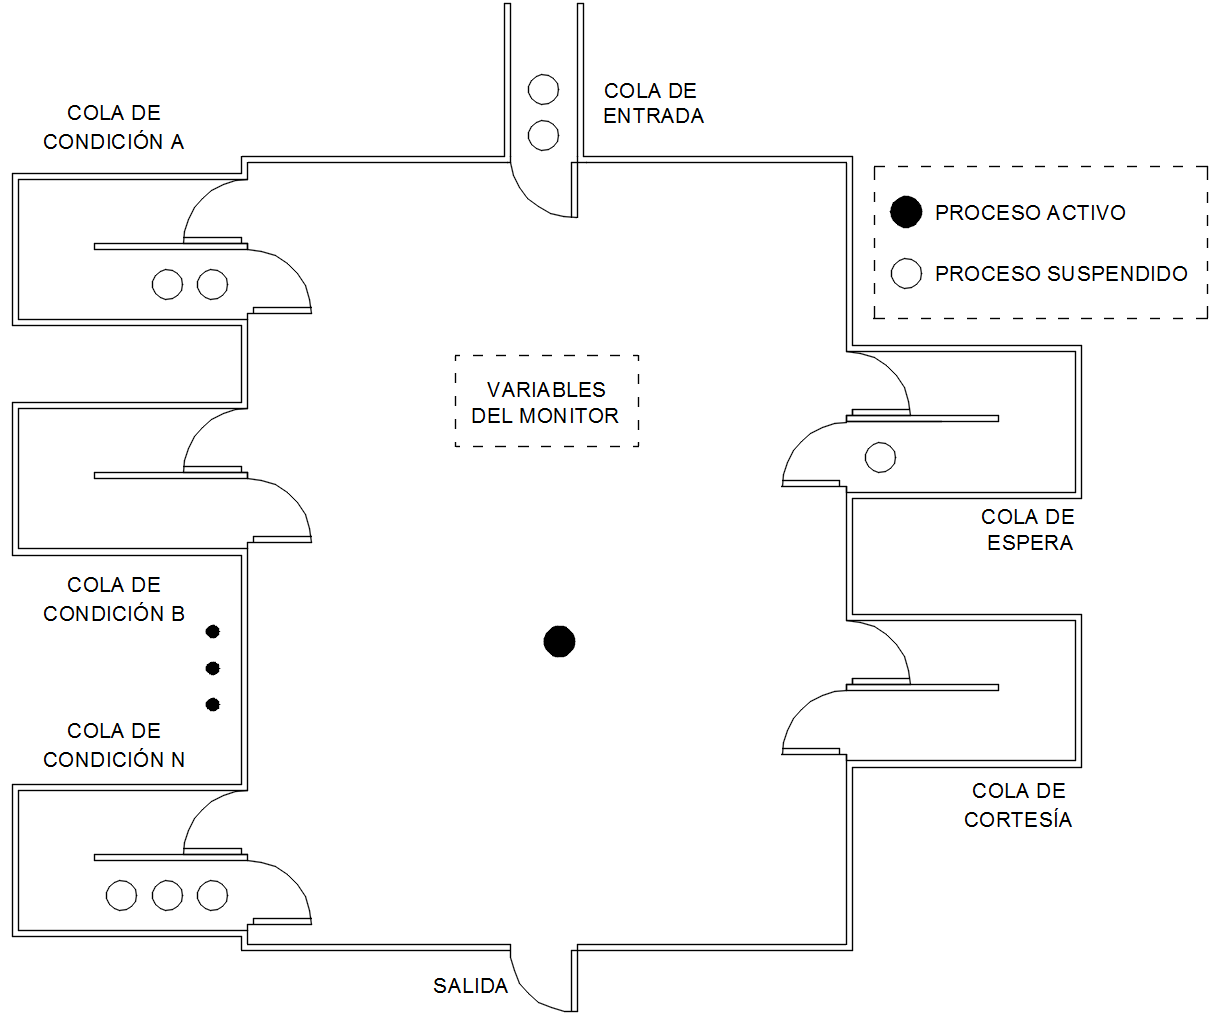
\includegraphics[height=100mm]{Monitor}
  \caption{Estructura de un Monitor de Concurrencia}
  \label{fig:monitor01}
\end{figure}

\paragraph{Cola de cortesía:}
Cuando un proceso libera a otro de mayor prioridad, tiene la opción de cederle
su lugar en el monitor. Si decide hacer esto, debe esperar fuera del monitor
para luego reanudar su ejecición dentro del mismo. Un posible lugar donde hacer
esta espera es la \textit{cola de cortesía}.
La cola de cortesía es una cola de espera que no está atada a ninguna condición.
Un proceso debería llamar a $signal$ sobre esta cola en lugar de liberar la
exclusión mutua de entrada si existe algún proceso esperando allí.

En la figura \ref{fig:monitor_cortesia} se observa la estructura de un monitor
con cola de cortesía.

\begin{figure}[h]
  \centering
  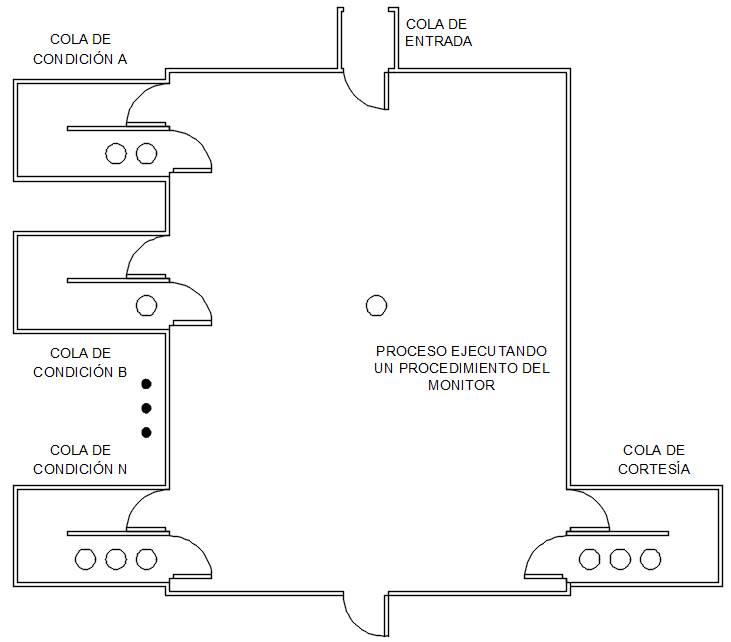
\includegraphics[height=100mm]{Monitor_Cortesia}
  \caption{Estructura de un Monitor de Concurrencia con Cola de Cortesía}
  \label{fig:monitor_cortesia}
\end{figure}

\subsubsection{Políticas de desbloqueo en monitores}
\label{politica_monitor}
El desbloqueo de un hilo suspendido por una llamada a $delay(X)$ sobre la
condición $X$ debe ser hecha por el hilo que produjo el cambio en la condición
$X$. Al analizar esta situación se desprenden múltiples formas de realizar esta
operación.

Para todos los siguientes casos, se considera que el proceso \textit{A}
desbloquea al proceso \textit{B} ejecutando $signal(x)$, condición sobre la que
\textit{B} se encuentra bloqueado inicialmente.

\paragraph{Desbloquear y continuar}
\textit{A} desbloquea a \textit{B} y continúa su ejecución dentro del monitor,
ya sea hasta terminar la llamada al procedimiento o hasta bloquearse en una cola
de condición. Una vez \textit{A} sale del monitor, \textit{B} ejecuta la
instrucción siguiente al $delay(x)$ que lo bloqueó.
En este punto, \textit{B} debe volver a verificar la condición que lo suspendió
porque no se puede garantizar que \textit{A} no la haya modificado luego de la
llamada a $signal(x)$.

\paragraph{Retorno forzado}
\textit{A} ejecuta una instrucción de salida del monitor ($return$ o $delay(n)$)
justo después de desbloquear a \textit{B}.
De esta manera, no es necesario que \textit{B} vuelva a comprobar su condición
ya que la exclusión mutua asegura que no fue modificada.

\paragraph{Desbloquear y esperar}
\textit{A} desbloquea a \textit{B} y automáticamente se agrega a la cola de
entrada del monitor.
Este enfoque tiene la ventaja de que \textit{B} no necesita comprobar su
condición de bloqueo una vez desbloqueado, pero \textit{A} cede su lugar en el
monitor y debe volver a competir por el ingreso para poder terminar su
ejecución.

\paragraph{Desbloquear y espera urgente}
Esta política soluciona el problema de inequidad de \textit{Desbloquear y
esperar}. Luego de desbloquear a \textit{B}, \textit{A} le cede su lugar en el
monitor, aunque en lugar de suspenderse en la cola de entrada del monitor lo
hace en la \textit{cola de cortesía}. De esta manera, el desbloqueo de
\textit{A} tendrá prioridad sobre el de cualquier proceso que intente entrar al
monitor.

\paragraph{Conclusión:}
Como con los semáforos, es posible cometer errores en la sincronización de los
monitores. La ventaja que tienen los monitores sobre los semáforos es que todas
las funciones de sincronización están confinadas dentro del monitor. De este
modo, es sencillo verificar que la sincronización se ha realizado correctamente
y detectar los fallos. Es más, una vez que un monitor está correctamente
programado, el acceso al recurso protegido es correcto para todos los procesos.
Con los semáforos, en cambio, el acceso al recurso es correcto sólo si
\textbf{todos los procesos} que acceden al recurso están correctamente
programados.\cite{SistOpStallings}
Por otro lado, las políticas de desbloqueo permiten especificar prioridades de
ejecución para los hilos, priorizando ya sea por orden de llegada o por algún
otro criterio. Si a su vez, se construye el monitor de forma modular para
cambiar la política de manera simple, se puede alterar la planificación de los
hilos de acuerdo a cada caso, según sea necesario. Si esto se intenta hacer
utilizando semáforos, resultaría mucho más difícil.
